\section*{A.2 Industrieroboter}

\subsection{Beschreiben Sie die Teilsysteme eines Industrieroboters und deren Funktion (S. 6, 20)}
\begin{description}
	\item[Kinematik:] bewegt die Fertigungseinrichtung zum Werkstück (räumliche Zuordnung zw. 
	  Werkstück und Fertigungseinrichtung); besteht aus Achsen, Antrieben, internen Sensoren, 
	  Effektoren;
	\item[Antrieb:] Übertragung/Umwandlung der Energie bis hin zum Effektor
	\item[Steuerung:] Umsetzung des Anwenderprogramms in eine Bewegung; Ein- und Ausgabeoperationen
	  zur Steuerung von Abläufen; Informationseingabe und -speicherung;
	\item[Messsystem:] Lage- und Geschwindigkeitmessungen der Achsen
	\item[Effektor:] Werstück-, Werkzeug-, Prüfmittelaufnahme
	\item[Externe Sensoren (optional):] Toleranzausgleich (zB: Kamera überprüft Abstand zum 
	  Werkstück); Lage- und Mustererkennung; 
\end{description}

\subsection{Beschreiben Sie die Bauformen von Industrierobotern (S.7)}
\begin{description}
\item[Portalroboter:] steife Struktur; rechteckiges oder quaderförmiges Industrieportal; 
  für große Arbeitsbereiche; Anw.: Transport von schweren Lasten, Verkettung von 
  Fertigungseinrichtungen;
\item[Roboter mit Lineararmen auf Schienen:] Lineararme meist in kartesischem Koordinatensystem
  angeordnet; Anw.: Einlegeoperationen, Punktschweißen;
\item[Schwenkarmroboter:] erste Achse ist Drehachse;
\item[Horizontalknickarmroboter (SCARA):] Achsen stehen senkrecht; Vorteil: billig, schnell, 
  genau!
\item[Vertikalknickarmroboter:] Achsen stehen horizontal (Abknicken in vertikaler Ebene 
  $\rightarrow$ Bremsen notwendig);
\end{description}
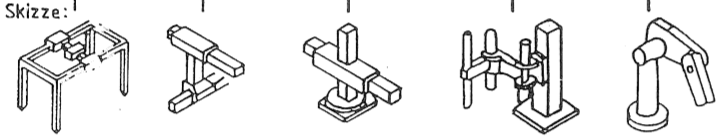
\includegraphics[width=\textwidth]{pics/bauarten}

\subsection{Nennen Sie Beispiele für Effektoren. Welche Vor- bzw. Nachteile haben pneumatische 
Greifer? (S.8,9,29-34)}
3 Arten: Greifer (Montage, Handhabung), Werkzeug (Schweißen, Schraubenzieher, Lackpistole), 
Prüfmittel (Sensoren)
\begin{description}
\item[Standardgreifer:] zwei ``Finger''/Backen, die ein Werkstück greifen; Hier kann mann noch
  zwischen \emph{pneumatischen} und \emph{elektromotorischen} Greifern unterscheiden:
  \begin{description}
    \item[pneumatisch:] + Greifkraft positionsunabhängig (konstant); - Nothaltevermögen durch
      zusätzliche Federn; + zentrieren Teile; - bewegliche Backen führen dazu, dass die 
      Position der Teile am Greifer nicht genau definiert ist;
    \item[elektromotorisch:] + Lageregelung (vgl. Nachteil bei pneumatisch) $\rightarrow$ 
      flexibler; + Greifkraft variabel (vgl. schwere vs. zerbrechliche Teile)
  \end{description}
\item[Sonderbacken:] + flexibler; Unterteilung in: Teilefamilienbildung (alle Werkstücke haben 
  eine best. Fläch wo der Backen das Teil aufnehmen kann), Stufengreifer (unterschiedliche
  Öffnungsweiten der Backen), Revolvergreifer (mehrere Teile auf einmal aufnehmen 
  $\rightarrow$ kürzere Taktzeiten), Greiferwechsel, Fingerwechsel
\item[Sauggreifer:] Werkstücke mit Unterdruck ansaugen; Anw.: Leiterplattenbestückung;
\item[Sonderbauformen:] Mehrfachgreifer, Kunststoffgreifer
\item[Werkzeugwechselsysteme:] Roboter wechselt die Greifer; - lange Taktzeiten;
\end{description}

\subsection{Nennen Sie Kriterien zur Auswahl eines Werkzeugwechselsystem. (S.34)}
Zulässige Kräfte und Momente, Anzahl der Steueranschlüsse, Anzahl der unterscheidbaren 
Werkzeuge, Einfahrtoleranzen, Spielfreiheit, Nothaltevermögen, Gewicht, Abmessungen, Preis

\subsection{Beschreiben Sie die verschiedenen Steuerungsarten von Industrierobotern. Zeichnen
  Sie eine Beispielskizze für die resultierende Bahn zwischen 2 Punkten bei einem 
  Industrieroboter mit 2 rotatorischen Achsen. (S.9,35-37)}
\begin{description}
\item[Punkt-zu-Punkt (PTP):] 2 Punkte gegeben $\rightarrow$ Winkel der Achsen werden 
  zurückberechnet (=Rückwärtskinematik) $\rightarrow$ Achsen bewegen sich unabhängig 
  voneinander zu den berechneten Winkeln (kann auch gleichzeitig/synchron erfolgen);
\item[Vielpunkt-Steuerung (MP):] Sollwerte/Punkte in festem Zeitraster vorgegeben (sonst
  wie PTP);
\item[Bahnsteuerung (CP):] mathematische Darstellung der Bahn, meist auch mit 
  Geschwindigkeitsvorgaben; alle Achsen bewegen sich synchron mit berechneten Achswinkeln;
\end{description}
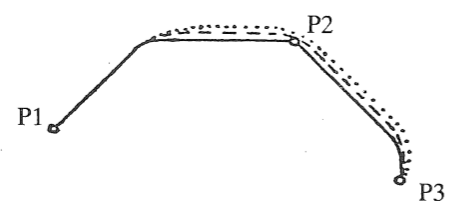
\includegraphics[width=.4\textwidth]{pics/ptp_bsp}

\subsection{Was versteht man unter Folgeprogrammierung? Beschreiben Sie Vor- und Nachteile im Vergleich zu Off-line-Programmierung.}
Folgeprogrammierung = (laut Prof.) Einstellverfahren: Punkte oder Bahn im Zeitraster einfach übernehmen (händisch, taktil, oder optisch positionieren)
\begin{itemize}
	\item[+] schnell
	\item[+] einfach
	\item[-] ungenau
\end{itemize}

\subsection{ Was versteht man unter Teach-In Programmierung? Beschreiben Sie Vor- und Nachteile im Vergleich zu Off-line-Programmierung. (S.10,38)}
\begin{description}
\item[Einstellverfahren:] Punkte oder Bahn im Zeitraster einfach übernehmen (händisch, taktil,
  oder optisch positionieren); + schnell; + einfach; - ungenau;
\item[Master-Slave:] Einstellen des Roboters mithilfe eines kleineren Master-Roboters 
  (händisch); 
\item[Teach-In:] Positionierung mit Handbediengerät; 
  - aufwendig; + genau (jeder Roboter ist anders! $\rightarrow$ hier: relative
  Genauigkeit miteinbezogen); - Roboter fällt für die Zeit des Teach-In's aus!
\item[Off-Line:] + textuelle Programmierung Off-Line (Roboter muss nicht für die Produktion 
  ausfallen); Simulation der Bewegung mit CAD-Daten; - ungenau, weil nur absolute Genauigkeit 
  des Roboters verwendet wird;
\end{description}
